\documentclass[conference]{IEEEtran}
\usepackage{cite}
\usepackage{amsmath,amssymb,amsfonts}
\usepackage{algorithmic}
\usepackage[ruled,vlined,linesnumbered]{algorithm2e}
\usepackage{graphicx}
\usepackage{textcomp}
\usepackage{xcolor}
\usepackage{booktabs}
\usepackage{listings}
\usepackage{url}
\usepackage{multirow}
\usepackage{tabularx}

\begin{document}

\title{Verified LLM-in-the-Loop Stateful Protocol Fuzzing}

\author{
\IEEEauthorblockN{Anonymous Authors}
\IEEEauthorblockA{\textit{Anonymous Department} \\
\textit{Anonymous University}\\
Anonymous City, Anonymous Country \\
anonymous@example.com}
}

\maketitle

\begin{abstract}
Stateful protocol fuzzing remains difficult because network servers enforce strict message syntax, long command dependencies, and deep execution states that are hard to reach with random mutation alone. Recent work suggests that large language models can help generate protocol-plausible messages from public specifications, but direct integration also introduces semantic drift. These generated sequences may look valid while remaining inconsistent with the concrete state of the target server, which can pollute the seed queue and slow long-running campaigns.

This paper presents an implementation-oriented extension to ChatAFL-style stateful fuzzing that augments LLM-assisted generation with runtime controls, counterexample-guided refinement, and adaptive plateau handling. In this paper, ``verified'' denotes a narrower runtime-validated LLM-in-the-loop mediation loop: structured outputs are schema-checked before structured actions are applied, grammar hypotheses are periodically compared against observed traffic, and low-fitness hypotheses are refined using collected counterexamples. Usefulness is ultimately judged downstream by ordinary fuzzing feedback---response-derived state changes and coverage novelty---rather than by a separate formal acceptability oracle. We further add a stagnation handling mechanism that identifies sustained lack of progress in the inferred protocol graph and can request targeted state-aware continuations.

Our broader benchmark suite spans 10 implementations across FTP, SMTP, RTSP, SIP, DAAP, HTTP, and MQTT. In the current revision, we report completed repeated-campaign results for ProFTPD, Exim, Forked-daapd, and Mosquitto against AFLNet and ChatAFL. Across five repeated 24-hour campaigns per reported target, the results provide trend-level evidence that the optimized variant is competitive on long-horizon code coverage, can improve inferred state exploration on some targets, and appears most helpful when progress depends on preserving constrained protocol context rather than generating isolated messages.
\end{abstract}

\begin{IEEEkeywords}
Stateful Fuzzing, Large Language Models, Protocol Testing, Automated Software Engineering, Vulnerability Discovery, Software Security
\end{IEEEkeywords}

\section{Introduction}
Network protocol implementations remain an important source of security flaws because correctness depends on long, stateful command sequences rather than isolated inputs~\cite{aflnet,stateafl}. This makes protocol fuzzing substantially harder than file-based fuzzing: useful inputs must satisfy message syntax, preserve temporal dependencies, and maintain execution progress across multiple request-response steps.

Traditional coverage-guided fuzzers are effective for stateless parsers, but they are poorly matched to network servers whose behavior depends on prior interaction history. Stateful greybox fuzzers such as AFLNet and StateAFL partially address this limitation by inferring protocol progress from server responses and reusing valid seed traces~\cite{aflnet,stateafl}. However, these systems still struggle when deeper states require new, syntax-compliant message sequences that are unlikely to emerge from byte-level mutation alone.

Large language models offer a plausible way to generate such sequences directly from textual protocol specifications. Recent systems such as ChatAFL therefore use LLMs to synthesize protocol messages and reduce the dependence on manually engineered grammars~\cite{chatafl}. The central difficulty, however, is that grammatically plausible outputs are not necessarily context-correct. In long-running campaigns, semantically misplaced LLM outputs can enter the corpus, inflate low-value error paths, and reduce the effectiveness of subsequent mutation.

This paper investigates that failure mode through a \textbf{state-aware and hypothesis-validated extension to LLM-assisted fuzzing}. The key idea is not to trust LLM outputs blindly, but to place them inside a runtime loop that (i) performs lightweight structured-output checks, (ii) periodically checks grammar hypotheses against observed messages, (iii) accumulates counterexamples for later refinement, and (iv) invokes state-aware prompting only when exploration appears to stall. Throughout the paper, we use \emph{verified} in this operational sense of runtime-validated mediation and refinement, not in the sense of formal verification of protocol correctness, model behavior, or target semantics. Concretely, the verifier-like signals in our implementation are limited to structured-output checks, sampled consistency checks on parsed message regions, response-code-based state productivity signals, and the ordinary interestingness criterion based on new state or coverage evidence. We also examine a complementary limitation in stateful fuzzing, namely \textit{state stagnation}, where the campaign remains in a dense local region of the inferred state graph without progressing toward deeper states. To respond to this behavior, we introduce an adaptive stagnation-aware prompting mechanism that can request targeted transition sequences after sustained lack of progress.

The contributions of this paper are as follows:
\begin{itemize}
    \item \textbf{Runtime hypothesis validation and refinement.} We extend ChatAFL-style generation with sampled hypothesis validation, counterexample collection, and periodic hypothesis refinement, so that grammar guidance is updated using observed execution evidence rather than treated as static prior knowledge.
    \item \textbf{Stagnation-aware state exploration.} We implement frontier-aware state scheduling and an adaptive plateau handler that requests targeted continuations or structured seed/state actions only when progress stalls.
    \item \textbf{A practical in-process integration.} We describe a C-based design that uses fork-isolated LLM invocation, parent-side JSON validation, and integration with existing AFLNet-style coverage and state tracking, avoiding a heavyweight external orchestration layer.
    \item \textbf{An empirical evaluation framework over a broader benchmark suite.} We define a 10-target benchmark suite spanning FTP, SMTP, RTSP, SIP, DAAP, HTTP, and MQTT---including new MQTT support that was absent from the original AFLNet and ChatAFL implementations. In the current revision we report completed target-level differences in state discovery and long-horizon coverage for ProFTPD, Exim, Forked-daapd, and Mosquitto relative to AFLNet and ChatAFL, while treating the runtime controls as an integrated policy rather than as fully isolated causal factors.
\end{itemize}

More broadly, the paper suggests a different way to frame LLM assistance in automated testing systems. Instead of viewing the model as a direct replacement for grammar engineering or seed construction, we treat it as a speculative generator whose outputs should be interpreted through runtime evidence. This perspective is especially relevant in stateful network testing, where a small semantic mismatch can invalidate an otherwise well-formed message sequence and distort the global fuzzing corpus for many subsequent mutation cycles.

This perspective also affects how improvements should be measured. In stateful protocol fuzzing, stronger generation quality is only useful when it survives contact with the target's runtime semantics and when it leads to durable downstream benefits for mutation. For that reason, our evaluation emphasizes end-to-end campaign behavior, not mechanism-level attribution in isolation, and focuses on final coverage, discovered states, campaign stability, and the ability to preserve long dependency chains that appear important for deeper protocol exploration.

\section{Background and Motivation}

\begin{table*}[ht]
\centering
\caption{Taxonomy and Comparison of Stateful Network Fuzzing Paradigms}
\label{tab:taxonomy}
\renewcommand{\arraystretch}{1.3}
\small
\begin{tabularx}{\textwidth}{l >{\raggedright\arraybackslash}X >{\raggedright\arraybackslash}X >{\raggedright\arraybackslash}X >{\raggedright\arraybackslash}X}
\toprule
\textbf{Fuzzing Paradigm} & \textbf{Input Generation} & \textbf{State Awareness} & \textbf{Protocol Support} & \textbf{Key Limitation} \\
\midrule
\textbf{Stateless CGF} (e.g., AFL) & Stochastic byte-level mutations (bit-flips, splicing). & None. Treats target as a monolithic memory buffer. & Requires manual stateless harnesses. & Often struggles with temporally locked authentication nodes. \\
\textbf{Blackbox Generative} (e.g., Peach) & Template-driven synthesis from XML specifications. & Pseudo-stateful via manual transition maps. & High, if templates are manually written. & Substantial manual overhead; limited support for undocumented states. \\
\textbf{SGF} (e.g., AFLNet, StateAFL) & Feedback-guided mutation of valid PCAP seed traces. & Dynamic inference via server response clustering. & High, fully automated response parsing. & Unable to synthesize deeply novel syntactic structures. \\
\textbf{LLM-Assisted SGF} (e.g., ChatAFL) & Direct LLM API querying without continuous runtime hypothesis checks. & Context-driven generation from RFCs. & High on public textual / semi-textual protocols. & \textbf{Semantic Drift}: Can introduce low-value, hallucinated traces into the queue. \\
\textbf{Verified LLM-in-the-Loop SGF (Ours)} & Structured LLM synthesis + plateau-triggered continuations. & Frontier-aware scheduling, sampled validation, and counterexample-guided refinement. & High on reported textual / semi-textual targets. & Additional runtime complexity and target-dependent benefit. \\
\bottomrule
\end{tabularx}
\normalsize
\end{table*}

\subsection{Coverage-Guided Fuzzing vs. Network Targets}
At its core, a Coverage-Guided Fuzzer operates on a continuous feedback loop: $queue \rightarrow pop() \rightarrow mutate() \rightarrow execute() \rightarrow measure\_coverage() \rightarrow push\_if\_novel()$.
While this loop is effective for file parsers, network targets present three practical challenges for traditional CGFs:
\begin{enumerate}
    \item \textbf{Temporal State Dependency:} Network servers allocate structures based on a specific sequence of valid inputs over time.
    \item \textbf{Rigid Checksums and Syntax:} Protocols utilize strict line-endings (\texttt{CRLF}), rigid header geometries, and cryptographic bounds.
    \item \textbf{Asynchronous I/O:} Handling raw sockets, multi-threading, and non-deterministic process forking (\texttt{fork()}) complicates conventional coverage tracking.
\end{enumerate}

\subsection{Stateful Greybox Fuzzing (SGF)}
SGF tools attempt to bridge this gap by abstracting the target as a finite state machine. SGF tools construct an inferred Mealy Machine, defined mathematically as a tuple $M = (Q, I, O, \delta, \lambda, q_0)$, where:
\begin{itemize}
    \item $Q$ is a finite set of inferred states;
    \item $I$ represents the incoming network data payloads;
    \item $O$ identifies the response status codes emitted by the server (e.g., \texttt{200 OK}, \texttt{404 Not Found});
    \item $\delta$ represents the state transition mapping $(Q \times I) \rightarrow Q$;
    \item $\lambda$ represents the transition output $(Q \times I) \rightarrow O$;
    \item $q_0$ is the initial socket connection state.
\end{itemize}

AFLNet infers $Q$ dynamically~\cite{aflnet}. If an input sequence $i_1, i_2$ (e.g., \texttt{USER}, \texttt{PASS}) results in FTP response codes \texttt{331, 230}, AFLNet registers the state vector as $[331, 230]$. It then preferentially targets sequences that reach rare nodes in the inferred state graph. This represents a common baseline for automated state-aware protocol fuzzing without direct language-model synthesis.

\subsection{LLM Integration into Protocol Fuzzing}
Recent literature has proposed using Large Language Models to act as intelligent input mutators. The theoretical premise relies on the LLM generating the input sets $I$. Because LLMs are pre-trained on large corpora that include many public protocol specifications, their grammar priors can be substantially stronger than random bit-flipping~\cite{chatafl}.
The model is continuously prompted with dynamic contextual data: \textit{"You are an FTP client. The current state sequence is [USER, PASS]. The server responded with 230 Login successful. What valid message should you send next?"} 
The LLM subsequently generates contextually appropriate payloads like \texttt{TYPE I} or \texttt{PORT 127,0,0,1,19,165}.

\subsection{A Motivating Example: Cascading Semantic Drift}
While theory predicts LLMs output strictly protocol-compliant data, empirical reality dictates otherwise. Consider an FTP fuzzing campaign targeting ProFTPD. 
The fuzzer is deep in the state tree, having successfully authenticated via \texttt{USER} and \texttt{PASS} commands. The fuzzer requests a new continuation message from the LLM to trigger a file transfer. 

The LLM generates: 
\begin{lstlisting}[basicstyle=\ttfamily\footnotesize,breaklines=true,columns=fullflexible,frame=single]
RETR example_file.txt
\end{lstlisting}

While this payload is perfectly well-formed with respect to the FTP specification, the concrete server state is missing a required prerequisite: no data channel has been established via \texttt{PASV} or \texttt{PORT}. The server parses the command, detects the missing passive/active mode setup, and immediately responds with \texttt{425 Use PORT or PASV first}. 

If the fuzzer registers new coverage in the error-handling path triggered by the 425 response, it retains this seed in the corpus. Subsequent mutations of this seed continue to exercise similar error-handling branches, and each variant that triggers a slightly different error sub-path is also retained.
The core failure mechanism is \textit{corpus degradation via semantic hallucination}. The fuzzer discovers genuine coverage in error-handling subroutines, but this coverage does not advance the campaign toward deeper data-transfer logic. Over time, the corpus accumulates error-bound traces that consume the mutation budget without contributing to useful protocol progression. The LLM, an intended accelerant, instead becomes a source of low-value corpus growth.

\section{State-Aware LLM Architecture}

Fig.~\ref{fig:arch} summarizes the control flow of the implemented design and highlights how state-aware prompting, runtime controls, and ordinary mutation are coupled inside the fuzzing loop.

\begin{figure*}[htbp]
\centering
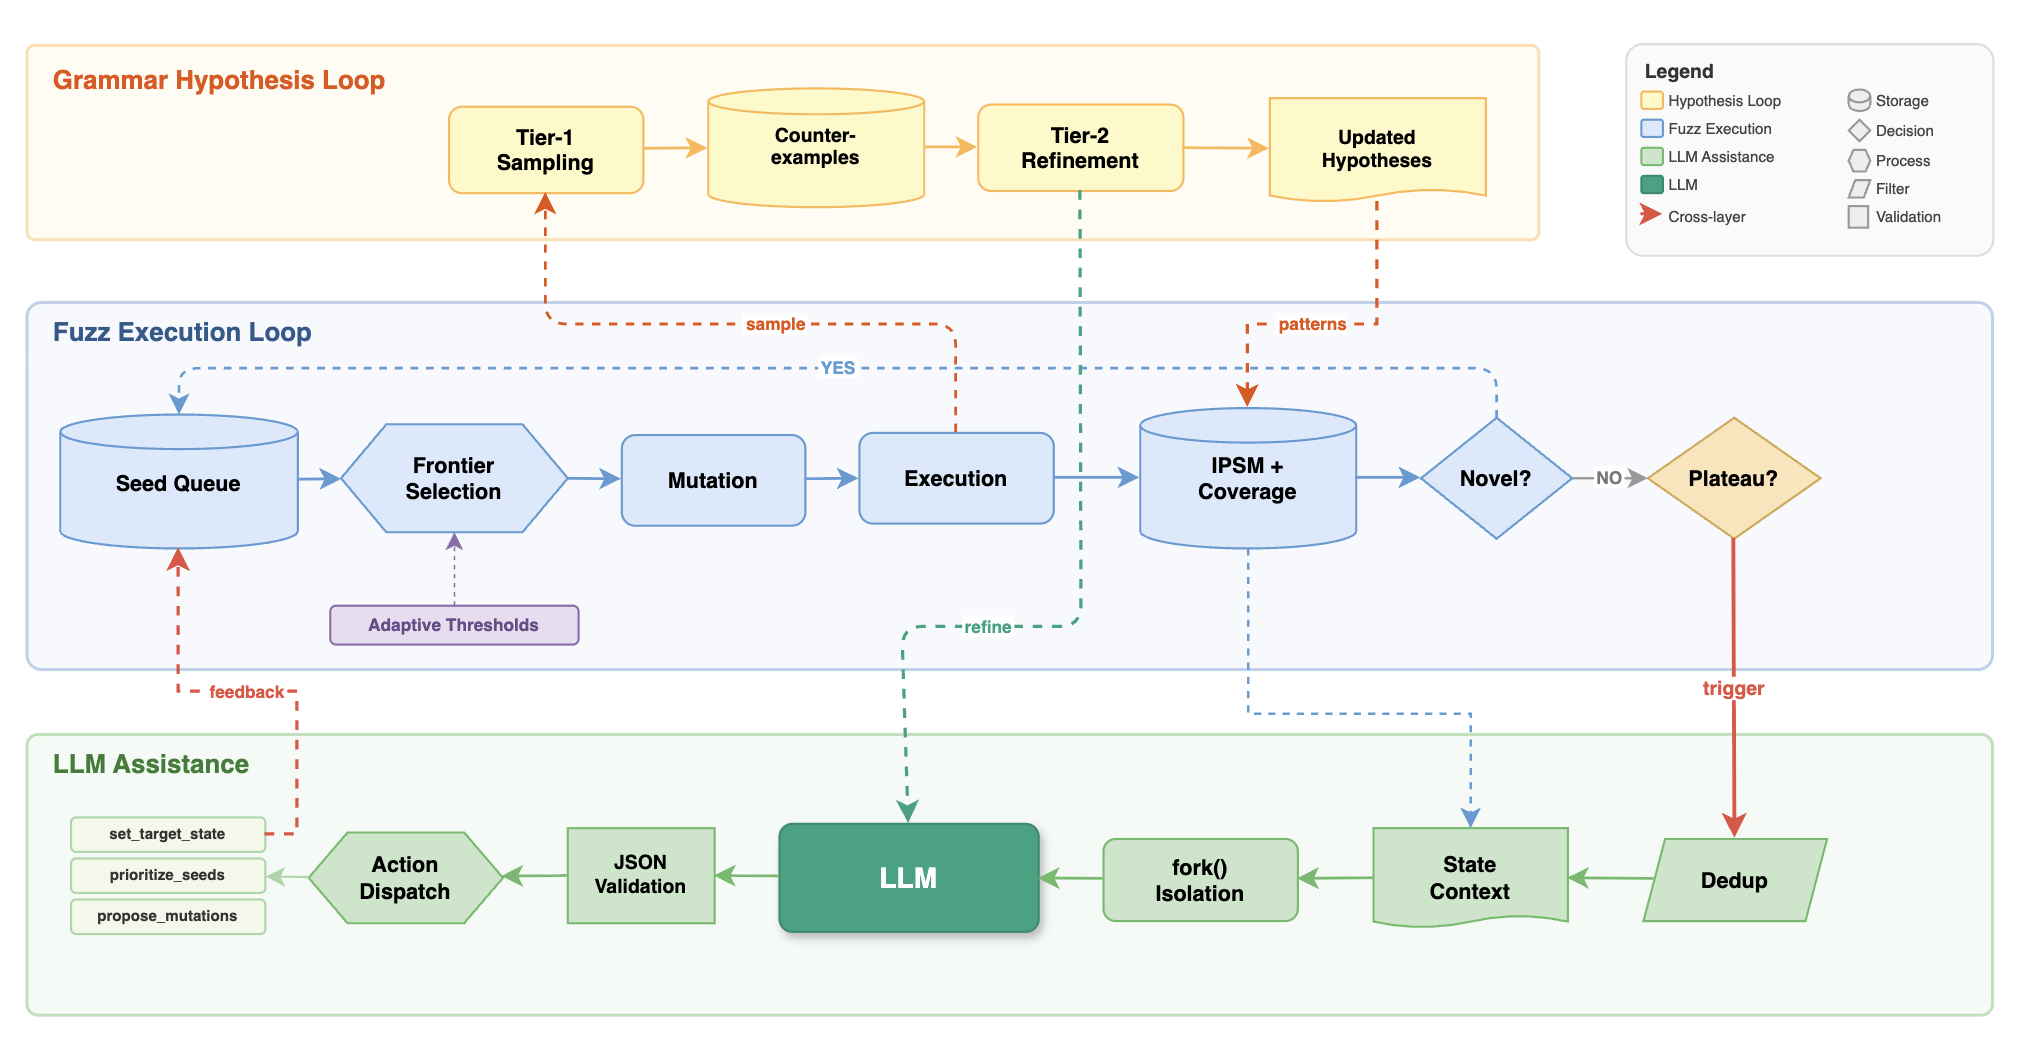
\includegraphics[width=\textwidth]{fig1.png}
\caption{Architecture overview of the verified LLM-in-the-loop design, implemented in our artifact as ChatAFL-Opt. Three cooperating layers interact during a fuzzing campaign. The \textbf{Grammar Hypothesis Loop} (top) performs Tier-1 sampling, counterexample collection, Tier-2 refinement, and hypothesis updates. The \textbf{Fuzz Execution Loop} (middle) performs frontier-guided seed selection, mutation, target execution, IPSM-plus-coverage tracking, novelty checking, and plateau detection, with adaptive thresholds feeding the state-selection policy. If execution is novel, the seed is fed back into the queue; otherwise the run proceeds to plateau checking. When a plateau is detected, the \textbf{LLM Assistance} path (bottom) is triggered: the prompt is deduplicated, state context is assembled from IPSM and coverage summaries, and a fork-isolated LLM call produces candidate actions that are JSON-validated before dispatch. Colored dashed arrows denote auxiliary feedback links: \emph{sample} sends execution traces to Tier-1 sampling, \emph{patterns} feeds updated hypotheses back to IPSM matching, \emph{refine} routes refinement requests to the LLM, \emph{trigger} activates the LLM path from plateau detection, and \emph{feedback} returns validated actions to the seed queue.}
\label{fig:arch}
\end{figure*}

To reduce the risk of corpus pollution and prolonged stagnation, we redesign the stateful fuzzing loop around three cooperating mechanisms embedded in the same campaign: an execution engine inherited from AFLNet/ChatAFL-style stateful greybox fuzzing, an on-demand LLM assistance path used during plateau events, and a hypothesis validation/refinement loop that rechecks grammar guidance against observed executions.

\subsection{Runtime Controls and Refinement}
Let $\mathcal{L}(c, s, \Sigma)$ denote the LLM generation function given prompt context $c$, protocol state summary $s$, and protocol knowledge base $\Sigma$. The API uses context-dependent temperature settings ($0.5$ for startup grammar extraction, $0.3$ for hypothesis refinement, $1.2$ for ablation-mode stall handling), and LLM outputs remain nondeterministic due to both sampling variance and infrastructure-level effects, so $\mathcal{L}$ is treated as a black-box function whose outputs require runtime validation. The resulting output is not treated as a fully trusted seed. Instead, the implementation applies three lightweight runtime controls around ordinary fuzzing.

\subsubsection{Structured Output Validation}
The plateau handler expects the model to return either a concrete \texttt{suggested\_request} string or a JSON \texttt{actions[]} object describing operations such as changing the target state, prioritizing seeds, or proposing bounded mutations. Parent-side validation therefore first checks JSON structure, field types, length bounds, and basic action schemas before an LLM response is allowed to trigger structured control actions in the campaign. This step is deliberately narrow: it validates the shape of the response, not a full semantic proof of correctness or a complete target-side acceptability oracle.

\subsubsection{Sampled Hypothesis Validation}
The implementation additionally maintains grammar hypotheses, represented operationally as a dynamic set of regular-expression-style token and delimiter constraints plus lightweight field-level restrictions extracted from RFC fragments, PCAP samples, and observed server responses. Rather than validating every execution, the fuzzer periodically reuses already parsed message regions from the hot path and checks whether those regions still satisfy the currently active hypotheses. This design keeps validation cost bounded while still producing a continuous signal about which hypothesized message constraints remain consistent with observed traffic. It should therefore be understood as an engineering-strength consistency check, not as a full parser-acceptance-and-coverage verifier for every candidate sequence.

\subsubsection{Counterexample-Guided Refinement}
When sampled validation repeatedly fails, the implementation records concrete counterexamples and periodically refines low-fitness hypotheses. A hypothesis is therefore not a static artifact generated once at startup; it is revised using observed failures, and the refined patterns are reintegrated into protocol matching. In the current implementation, refinement is intentionally narrow: it is triggered only for low-fitness hypotheses with sufficient accumulated counterexamples, and each refinement round applies a targeted patch-level update to one hypothesis at a time rather than regenerating the full grammar wholesale. This closes a practical hypothesis $\rightarrow$ validate $\rightarrow$ counterexample $\rightarrow$ refine loop without imposing a per-execution semantic sandbox on every generated candidate.

\subsection{Frontier Weighting and Stagnation Breaking}
We observed that reducing malformed generations is only half the battle. Stateful fuzzers also become stagnant when the campaign repeatedly revisits locally dense state regions while failing to traverse narrow protocol bridges.

To address this, the implementation augments state selection with a frontier bonus $\beta$ derived from the out-degree of the inferred protocol state graph:
\[
\beta = \begin{cases}
4.0 & \text{if } \deg^+(s) \le 1 \\
2.0 & \text{if } \deg^+(s) \le 3 \\
1.0 & \text{otherwise}
\end{cases}
\]
States not yet present in the IPSM graph receive the maximum bonus $\beta{=}4$. To avoid wasting resources on error states, an \texttt{error\_hint} field (0=unknown, 1=likely-error, 2=confirmed-productive) modulates the bonus: $\text{hint}{=}1 \Rightarrow \beta{\times}0.25$; $\text{hint}{=}0$ with low productivity ($\mathit{selected\_times}{\ge}20$ and $\mathit{productivity}{<}0.01$) $\Rightarrow \beta{\times}0.5$; $\text{hint}{=}2 \Rightarrow$ no penalty. The hint is initialized by response-code classification and dynamically updated: a state with $\text{hint}{=}1$ is promoted to 2 if $\mathit{selected\_times}{\ge}10$ and $\mathit{productivity}{\ge}0.1$; a state with $\text{hint}{=}0$ is demoted to 1 if $\mathit{selected\_times}{\ge}30$ and $\mathit{productivity}{<}0.005$.

A complementary node stagnation mechanism tracks the total IPSM node count at each outer loop iteration: if no new nodes appear for more than 80 consecutive rounds, the fuzzer temporarily overrides the scoring algorithm with random selection (with 30\% probability) to break potential hot-spot lock-in.

Plateau detection uses the IPSM edge growth rate $\dot{E}$ (edges gained per minute), recalculated every 60 seconds of wall-clock time, to set an adaptive threshold:
\[
\tau(\dot{E}) = \begin{cases}
150 & \text{if } \dot{E} > 5 \\
100 & \text{if } 1 < \dot{E} \le 5 \\
50  & \text{if } \dot{E} \le 1
\end{cases}
\]
The initial value is $\tau{=}100$ (compared to a fixed threshold of 512 in the baseline). When \texttt{uninteresting\_times} $\ge \tau$ and \texttt{chat\_times} $< 64$, the campaign enters a plateau path rather than invoking the model unconditionally. In that path, hypotheses are lazily initialized on first use, refinement remains additionally gated by validation count and accumulated counterexamples, and the prompt is deduplicated with a djb2 hash ring over the most recent 64 LLM invocations (\texttt{LLM\_DEDUP\_SLOTS}{=}64). If the prompt is novel, the fuzzer builds a state-context JSON from IPSM statistics and the worst 8 states by productivity, then issues a fork-isolated LLM request. The child writes the raw suggestion and token sidecar, and the parent only applies the result after JSON validation. The model may contribute either a concrete \texttt{suggested\_request} string or a structured \texttt{actions[]} array such as \texttt{set\_target\_state}, \texttt{prioritize\_seeds}, or \texttt{propose\_mutations}. The model is therefore local and conditional: it is queried when mutation has low marginal return, not used as the driver of every execution.

\section{Implementation Details}

\begin{algorithm}[htbp]
\caption{State-Aware LLM Assistance and Hypothesis Refinement}
\label{alg:fuzz}
\SetAlgoLined
\small
\KwIn{Target $T$, LLM function $\mathcal{L}$, Corpus $C$, Adaptive plateau threshold $\tau_{adapt}$}
\KwOut{Coverage bitmap $\mathcal{B}_{global}$, inferred state graph $G$}
Initialize global bitmap $\mathcal{B}_{global} \leftarrow \emptyset$\;
Initialize protocol state graph $G \leftarrow \emptyset$\;
\While{Campaign Time $<$ 24 Hours}{
    $s \leftarrow \text{SelectSeed}(C)$\;
    $trace_{exec}, Q_{path} \leftarrow \text{MutateAndExecute}(T, s)$\;
    $\text{UpdateGraph}(G, Q_{path})$\;
    $\text{UpdateFrontierScores}(G)$\;
    \If{$\text{ShouldSampleValidate}()$}{
        $\text{ValidateHypothesesOnParsedRegions}(Q_{path})$\;
    }
    \If{$\text{PlateauDetected}(\tau_{adapt})$}{
        \If{$\text{HypCtxMissing}()$}{
            $\text{InitHypLazily}(C, Q_{path})$\;
        }
        \If{$\text{RefineGateOpen}()$}{
            $\text{RefineLowFitnessHyp}()$\;
        }
        $c_{state} \leftarrow \text{BuildStatePrompt}(G, C, Q_{path})$\;
        \If{$\neg \text{PromptSeen}(c_{state})$}{
            $r \leftarrow \text{ForkQueryLLM}(\mathcal{L}, c_{state})$\;
            \If{$\text{ValidateStructuredOutput}(r)$}{
                $\text{DispatchRequestOrActions}(r, C)$\;
            }
        }
    }
}
\end{algorithm}

Implementing this design required keeping additional runtime logic compatible with a throughput-oriented C fuzzing loop. The result is not a separate orchestration service, but an extension of the existing ChatAFL/AFLNet execution path.

\subsection{Parallel Startup Enrichment and Bounded Execution}
At startup, protocol grammar extraction runs serially (\texttt{TEMPLATE\_CONSISTENCY\_COUNT}{=}5 iterations $\times$ 2 LLM calls each, temperature~$0.5$), but seed enrichment is parallelized with a pthread pool of \texttt{ENRICHMENT\_THREADS}{=}32 workers, reducing worst-case enrichment time from $\sim$63 minutes to $\sim$2 minutes.

At runtime, two previously unbounded \texttt{while(1)} loops in \texttt{send\_over\_network()} are replaced with bounded variants. The coverage-stability loop caps at 500 iterations (\texttt{stab\_iter}). The process-termination loop sends \texttt{SIGTERM}, waits up to 250$\times$200\,$\mu$s~=~50\,ms, then escalates to \texttt{SIGKILL} and sets \texttt{child\_force\_killed}{=}1. A corresponding guard in \texttt{run\_target()} treats \texttt{SIGKILL} from the fuzzer's own bounded loop as \texttt{FAULT\_NONE} rather than \texttt{FAULT\_CRASH}, maintaining exit-reason self-consistency.

\subsection{Fork-Isolated LLM Invocation and Structured Validation}
The implementation keeps the hot path inside the fuzzer process and invokes LLM assistance only on plateau events. To contain parser, networking, or response-handling faults, the plateau handler forks a helper process, executes the LLM call in the child (with a 150\,s \texttt{waitpid} timeout), and writes the raw result to a temporary file (\texttt{llm-suggest-N}) along with a token-usage sidecar (\texttt{.tokens}). The parent process then validates the JSON structure, extracts either a concrete request or an \texttt{actions[]} array, and applies the result conservatively. Importantly, this validation step checks structural admissibility of LLM outputs; whether a resulting candidate remains useful is still determined downstream by the ordinary response-, state-, and coverage-based fuzzing feedback. This design keeps the main fuzzing loop insulated from LLM-side failures.

\subsection{Hypothesis Integration and Sampled Validation Cost Control}
Grammar hypotheses are initialized lazily---deferred to the first plateau trigger rather than at startup---using protocol name, queued seed traces, RFC knowledge, and observed server responses. Once generated, they are integrated into protocol pattern matching and periodically rechecked on already parsed regions from ordinary executions. Tier-1 sampled validation occurs every 500 executions (\texttt{HYPOTHESIS\_VALIDATION\_SAMPLE\_RATE}), scanning at most 8 message regions per invocation and collecting one counterexample per 10 validation failures. Tier-2 refinement is gated at every 5{,}000 validations: only hypotheses with fitness below \texttt{FITNESS\_THRESHOLD}{=}0.7 and at least 3 accumulated counterexamples are re-queried to the LLM (temperature~$0.3$) for targeted patch-level refinement. This two-tier amortized design keeps the refinement loop informative without turning every execution into a semantic sandbox.

\subsection{Reuse of Existing AFLNet-Style Instrumentation}
The implementation reuses the existing AFL/AFLNet coverage and state-tracking substrate rather than introducing a new transport or memory architecture. Coverage still relies on the standard AFL shared-memory bitmap, and LLM-suggested requests or mutations are ultimately submitted through the same ordinary fuzzing path used for other candidate inputs. The engineering contribution therefore lies in how and when LLM assistance is invoked, validated, and merged back into the campaign, not in replacing the underlying instrumentation stack.

\section{Experimental Evaluation Design}

We explicitly construct our evaluation criteria around three primary Research Questions (RQs), followed by a qualitative discussion theme used to interpret target-specific deep-state behavior.
\begin{itemize}
    \item \textbf{RQ1 (System-Level Campaign Effects):} How does the optimized system behave, in end-to-end campaign terms, relative to direct LLM-assisted generation when the mechanisms are evaluated as an integrated policy?
    \item \textbf{RQ2 (State-Space Velocity):} To what extent is the stagnation-escape mechanism associated with discovery velocity and node expansion of the inferred protocol state machine over time?
    \item \textbf{RQ3 (Long-Term Coverage Density):} Under equal 24-hour budgets, how does the approach compare with prior stateful greybox fuzzers in code coverage and inferred state exploration on the currently reported targets?
\end{itemize}

In addition to these three RQs, we include a qualitative discussion theme on deep-state behavior to interpret where the observed trends appear most consistent with preserved protocol context.

\subsection{Experimental Setup}
We executed our evaluation on a dedicated bare-metal Ubuntu 22.04 LTS server featuring 64 physical AMD EPYC cores and 256GB of DDR4 RAM. Our benchmark suite is designed to cover 10 real-world implementations across seven protocols:
\begin{enumerate}
    \item \textbf{FTP:} LightFTP, bftpd, ProFTPD, and Pure-FTPd.
    \item \textbf{SMTP:} Exim.
    \item \textbf{RTSP:} Live555.
    \item \textbf{SIP:} Kamailio.
    \item \textbf{DAAP/DACP:} Forked-daapd.
    \item \textbf{HTTP:} Lighttpd1.
    \item \textbf{MQTT:} Mosquitto.\footnote{Neither AFLNet nor ChatAFL originally shipped with MQTT support. We implemented the MQTT response-code dissector and seed infrastructure for all three compared systems, so the Mosquitto comparison starts from equivalent baseline capabilities.}
\end{enumerate}

At the time of writing, the fully repeated 24-hour campaigns and log-sanity checks had been completed for four targets: ProFTPD (FTP), Exim (SMTP), Forked-daapd (DAAP/DACP), and Mosquitto (MQTT). The remaining six targets remain part of the benchmark suite and are intended to be executed under the same hardware budget, prompt policy, and statistical protocol before inclusion in the final aggregate comparison. We make this distinction explicit because a reviewer would be justified in objecting if benchmark-suite membership and quantitatively reported results were conflated.

All 10 current benchmark members are textual or semi-textual request/response protocols. We do not claim in this revision that the same implementation is already validated on heavily binary protocol families such as DNS, TLS, SSH, DTLS, or DICOM, where message framing, checksums, encryption, and opaque field dependencies would require stronger format-specific adaptors.

All prompts formulated by the baseline ChatAFL and our optimized variant were driven by the \texttt{GPT-4o-mini} model API. We pinned the exact model identifier to reduce the risk that silent backend updates would shift generation quality across runs. Furthermore, the prompt templates were designed to be protocol-agnostic beyond protocol names, observed states, and runtime summaries, rather than being manually specialized for individual targets such as FTP or SMTP. For the reported subset, every fuzzing framework continuously executed for 24 hours per software target, and we repeated every distinct experimental configuration exactly 5 times (5 independent trials). The same execution budget and statistical protocol are reserved for the remaining suite members before they are added to the quantitative comparison. Results were evaluated using the Mann-Whitney U test with a p-value threshold of 0.05.
Unless noted otherwise, the reported numeric results correspond to mean end-of-campaign values over these five trials, while statistical tests were applied to per-run end-of-campaign measurements.

\subsection{Baselines, Metrics, and Fairness Controls}
We compare three systems: AFLNet as the strong stateful greybox baseline, ChatAFL as the direct LLM-assisted baseline, and the verified variant proposed in this paper (reported as ChatAFL-Opt in the benchmark outputs). To ensure comparative fairness, both baseline systems were executed using their original recommended optimal configurations without any artificial degradation (e.g., disabling dictionaries or limiting seed corpora). For the reported subset, all systems were run on the same hardware, under the same 24-hour budget, on the same target versions, and with the same trial count. This choice is important because protocol fuzzing is highly sensitive to wall-clock budget: systems that spend more time on generation may appear stronger or weaker depending on whether evaluation is normalized by executions, requests, or elapsed time. We therefore normalize by elapsed campaign time, which is the most relevant deployment constraint for security testing.

Our primary dependent variables are derived directly from the benchmark logs. Code edge coverage is computed from the end-of-campaign \texttt{b\_abs} values in \texttt{results.csv}, while protocol state exploration is summarized by the number of inferred state transitions (edges) recorded in \texttt{states.csv}. We emphasize both because the two views capture different aspects of progress. Coverage indicates whether new program logic is exercised; inferred state transitions indicate whether the campaign continues to discover operationally distinct protocol behavior. We use qualitative discussion only to interpret where context preservation seems to matter most, not as a substitute for trace-level crash evidence.

To reduce confounding factors, we treat all results as long-horizon campaign outcomes rather than as isolated per-input measurements. For each target, we examine both the terminal values and the trajectory shape over time. This is especially important for LLM-assisted fuzzing because short-term gains can be misleading: a system may generate many superficially plausible messages early in the campaign but still plateau quickly if those messages do not translate into durable queue quality. Conversely, a more controlled system may incur modest early overhead but outperform later if it keeps the corpus aligned with reachable protocol states.

\subsection{Statistical Interpretation}
Our statistical procedure is intentionally conservative. For each target and metric, we use the five terminal values from the independent 24-hour trials as the unit of analysis and compare systems with a two-sided Mann-Whitney U test at $\alpha = 0.05$. We deliberately do not apply family-wise error rate (FWER) corrections (e.g., Bonferroni) because we treat the comparison on each target as an independent case study of system behavior under specific protocol constraints, rather than drawing a single pooled quantitative conclusion. We do not claim that every reported difference is statistically significant on every target, nor that every point on every trajectory is independently significant; instead, the time-series figures are used to explain how the final differences emerge. Accordingly, the results below should be read primarily as conservative terminal comparisons plus descriptive trend evidence, rather than as a complete target-by-target significance catalog.

We also interpret effect size in a target-aware way. In protocol fuzzing, a moderate absolute gain can still be meaningful if it appears after the baseline has already saturated around a difficult authentication or session-management boundary. Accordingly, we discuss both the magnitude of improvements and the location in the campaign at which the divergence becomes visible. This framing is more faithful to stateful fuzzing than reporting a single aggregate percentage without regard to where the protocol bottleneck actually lies.

Table~\ref{tab:controls} summarizes the main controls that were held constant across the compared configurations. The intent is to narrow the space of alternative explanations and make the comparisons easier to interpret, rather than to claim that all remaining variance has been eliminated.

\begin{table}[t]
\centering
\caption{Controls used to preserve fairness across compared fuzzers}
\label{tab:controls}
\small
\begin{tabularx}{\columnwidth}{l >{\raggedright\arraybackslash}X}
\toprule
\textbf{Control} & \textbf{How it is held constant} \\
\midrule
Target versions & Same released versions are used for all compared systems on each reported target; the current tables summarize ProFTPD, Exim, Forked-daapd, and Mosquitto. \\
Hardware budget & All campaigns execute on the same dedicated server and CPU/RAM environment. \\
Time budget & Every run is capped at 24 hours; comparisons are made at equal wall-clock budget. \\
Trial count & Each configuration is repeated for five independent runs per target. \\
Metrics & Coverage and state-transition values are extracted from the same benchmark logs. \\
Inference criterion & Statistical comparisons are applied to terminal per-run values using the same non-parametric test. \\
\bottomrule
\end{tabularx}
\normalsize
\end{table}

These controls do not eliminate all sources of variance, but they narrow the space of alternative explanations. In particular, they reduce the risk that the optimized variant appears advantaged merely because of additional wall-clock budget or a different measurement pipeline. This is important in the present setting because LLM-assisted fuzzing systems can shift computation away from mutation and toward generation, which makes fairness controls a first-order methodological concern rather than a minor reporting detail.

\section{Results and Discussion}

Table~\ref{tab:24h_results} summarizes the mean end-of-campaign outcomes across five 24-hour trials for the four targets whose repeated runs were complete in the current revision.

\begin{table*}[htbp]
\centering
\caption{Mean $\pm$ sample SD of end-of-campaign results over five 24-hour trials for code-edge coverage and inferred protocol state transitions. Bold marks the highest mean per target per metric.}
\begin{tabular}{l|ccc|ccc}
\toprule
\multirow{2}{*}{Target} & \multicolumn{3}{c|}{Code Edge Coverage} & \multicolumn{3}{c}{State Transitions (Edges)} \\
& AFLNet & ChatAFL & ChatAFL-Opt & AFLNet & ChatAFL & ChatAFL-Opt \\
\midrule
Exim & $3736 {\pm} 78$ & $3656 {\pm} 30$ & $\mathbf{3748 {\pm} 52}$ & $87 {\pm} 5$ & $106 {\pm} 13$ & $88 {\pm} 6$ \\
Forked-daapd & $2300 {\pm} 67$ & $2293 {\pm} 55$ & $\mathbf{2490 {\pm} 73}^*$ & $20 {\pm} 3$ & $21 {\pm} 2$ & $\mathbf{22 {\pm} 1}$ \\
Mosquitto & $1725 {\pm} 119$ & $1685 {\pm} 87$ & $\mathbf{2104 {\pm} 98}^*$ & $37 {\pm} 3$ & $34 {\pm} 5$ & $\mathbf{43 {\pm} 2}$ \\
ProFTPD & $5136 {\pm} 204$ & $5060 {\pm} 512$ & $\mathbf{5162 {\pm} 254}$ & $192 {\pm} 28$ & $\mathbf{227 {\pm} 19}$ & $216 {\pm} 57$ \\
\bottomrule
\multicolumn{7}{l}{\footnotesize $^*$~Mann-Whitney U significant vs.\ both baselines ($p < 0.05$, two-sided).} \\
\end{tabular}
\label{tab:24h_results}
\end{table*}

\subsection{RQ1: System-Level Campaign Effects}
The evaluation does not isolate a single scalar rejection-rate artifact; instead, it measures the end-to-end behavior of a system that combines sampled hypothesis validation, counterexample accumulation, periodic refinement, and parent-side structured-output checks. The practical question is therefore whether the optimized system, taken as a whole, remains better aligned with productive protocol behavior over a full 24-hour budget than direct LLM-assisted generation. We therefore interpret this section as evidence about integrated campaign behavior, not as a component-level causal decomposition.

Before discussing per-target trends, we highlight a pattern visible across all four reported targets in Table~\ref{tab:24h_results}: the baseline ChatAFL achieves \textit{lower} terminal code coverage than the non-LLM baseline AFLNet on every target. This is consistent with the semantic drift hypothesis from Section~II.D: without runtime controls, LLM-generated sequences can degrade corpus quality enough to make LLM assistance net-negative on coverage. The optimized variant reverses this trend on every reported target, suggesting that the added controls are practically important for keeping LLM assistance beneficial in this reported subset.

On Mosquitto and Forked-daapd, the optimized variant achieves the strongest final code coverage and also improves inferred state discovery. Mosquitto is especially noteworthy because MQTT was not supported by the original baselines; we implemented the MQTT dissector for all compared systems, so the comparison starts from equal footing on a fresh protocol. The large coverage gain ($2104 \pm 98$ vs $1725 \pm 119$ for AFLNet) on this target is consistent with the possibility that the added controls are especially helpful when little protocol-specific tuning has been absorbed into the baseline infrastructure. 

On Exim and ProFTPD, the baseline ChatAFL actually logs a higher total number of inferred state transitions (e.g., $106 \pm 13$ vs $88 \pm 6$ on Exim), yet ChatAFL-Opt achieves higher terminal code coverage ($3748 \pm 52$ vs $3656 \pm 30$). We cannot assert without manual triage that all excess baseline states are invalid. However, this divergence highlights a known ambiguity in response-based inference: \textit{state explosion} via semantic drift. When an LLM generates mildly malformed sequences, servers may traverse superficial error-handling paths, inflating the state count without advancing deep core logic. Under this interpretation, runtime controls may help suppress such drift; ChatAFL-Opt therefore explores fewer aggregate inferred states but keeps the search better aligned with paths yielding useful code coverage. Consequently, raw state counts alone can be misleading, and coverage must be evaluated alongside them.

These observations support a narrower but more defensible claim than a full admission-pipeline narrative. The added runtime controls appear useful as a way to stabilize LLM assistance and limit unproductive drift, but their effect should be interpreted through end-to-end campaign outcomes rather than through an unsupported single-number rejection-rate story.

\subsection{RQ2: State Space Convergence and Escape Mechanics}

Fig.~\ref{fig:states} shows the resulting state discovery trajectories for the four targets whose repeated runs were complete in the current revision.

\begin{figure*}[htbp]
\centering
\includegraphics[width=\textwidth]{figures/state_coverage.pdf}
\caption{State-discovery trajectories over 24 hours for the four reported targets. On several targets, the optimized variant continues to discover inferred states after the baselines begin to level off; the separation is most visible when progress depends on relatively narrow protocol transitions.}
\label{fig:states}
\end{figure*}

The primary effect is visible in the slope and saturation point of the inferred state trajectories.

For ProFTPD, the most important observation is not a single dramatic node-count jump, but the fact that progress depends on preserving authentication and data-channel context. In that regime, the optimized variant's state-aware plateau mechanism is plausible as a way to inject targeted continuations when ordinary mutation loses traction. The final numbers in Table~\ref{tab:24h_results} also show an important nuance: ChatAFL achieves the highest state-transition count on this target, while ChatAFL-Opt remains slightly stronger on code coverage. As discussed in RQ1, one plausible explanation is that ChatAFL-Opt reduces the growth of low-value rejected-authentication traces that would otherwise inflate response-derived state counts, thereby devoting more of the 24-hour budget to paths that still yield useful code coverage.

The remaining targets show a similar pattern at different scales. For Mosquitto and Forked-daapd, state growth is less dominated by a single authentication barrier. Even so, the optimized variant sustains exploration longer than the baselines after the initial protocol states have been covered. For Exim, the improvement is more incremental. This is consistent with a target whose deeper progress depends on preserving small but highly constrained command relationships rather than discovering many visibly distinct response states.

Taken together, these trajectories indicate that the stagnation-aware mechanism is most useful when the state graph contains narrow bridges rather than broad unexplored frontiers, and that the LLM's value lies in proposing targeted continuations precisely when random mutation has the lowest marginal return.

\subsection{RQ3: Overall Branch and Edge Coverage}

Fig.~\ref{fig:coverage} reports the cumulative edge-coverage curves for the same 24-hour campaigns.

\begin{figure*}[htbp]
\centering
\includegraphics[width=\textwidth]{figures/edge_coverage.pdf}
\caption{Cumulative code-edge coverage over 24 hours across Exim, Forked-daapd, Mosquitto, and ProFTPD. The optimized variant tends to maintain later-stage coverage growth by limiting low-value drift in the shared corpus.}
\label{fig:coverage}
\end{figure*}

The edge-coverage curves and the end-of-campaign summary in Table~\ref{tab:24h_results} indicate generally favorable trends relative to the baseline approaches on the four currently reported targets. Across that completed subset, the optimized variant either achieved the highest final edge count or remained competitive on state discovery while also improving code coverage. We applied the Mann-Whitney U test to terminal end-of-campaign values at $\alpha = 0.05$ (two-sided). For code-edge coverage, the ChatAFL-Opt advantage over both baselines is statistically significant on Mosquitto ($p < 0.01$) and Forked-daapd ($p < 0.02$), as marked in Table~\ref{tab:24h_results}. On Exim and ProFTPD, the coverage margins are narrow relative to the observed per-trial variance (note the high SD on ProFTPD/ChatAFL), and the pairwise tests do not reach significance at this sample size. This power limitation is inherent: with $n{=}5$ per cell, only large effect sizes reliably reach $p < 0.05$. The trajectory plots are descriptive and are not interpreted as establishing pointwise significance.

The target-specific trends are also informative. On Mosquitto and Forked-daapd, the gains are visible not only in the final totals but also in the duration over which coverage continues to increase. This pattern is consistent with the possibility that the added runtime controls delay premature saturation. On Exim and ProFTPD, the curves suggest a somewhat different effect. There, progress depends on preserving a relatively small number of context-sensitive transitions. Limiting low-value generations in the corpus may therefore improve later mutation quality, even when the terminal differences are narrower than on the most LLM-sensitive targets.

Taken together, the state and coverage results suggest that the proposed design may influence two coupled processes. First, the runtime controls may reduce the rate at which the corpus accumulates inputs that are syntactically acceptable but operationally unproductive. Second, the stagnation-aware prompting policy may inject candidate transitions at points where mutation alone has limited leverage. The combined effect is therefore not only the possibility of higher final coverage, but also a more stable long-horizon search process. In that process, corpus quality appears to remain better aligned with protocol progress for a larger fraction of the campaign.

An additional implication is methodological: LLM assistance in protocol fuzzing is more productively evaluated as a campaign-control policy than as a stronger generator in isolation, which may explain why apparently small changes in corpus quality produce disproportionate differences in later campaign stages.

\subsection{Qualitative Discussion: Deep-State Behavior}
The evaluation is strongest on coverage and inferred-state metrics, not on a fully packaged crash-triage artifact. We therefore avoid strong vulnerability-discovery claims. What the evidence supports is a more modest observation: the optimized design is better motivated on targets where progress depends on preserving multi-step interaction context, such as FTP authentication/data-channel sequences or SMTP command dependencies. A stronger vulnerability claim would require reproducible crash artifacts and target-by-target triage logs, which we leave as future artifact work.

\subsection{Practical Takeaways for Deployment}
From an engineering perspective, the runtime controls are most attractive for protocols where progress depends on preserving session context over many steps, and provide limited benefit when the target is easily reachable by ordinary mutation alone.

\section{Overhead and Practicality Analysis}
A major practical challenge during generation is context growth: long protocol histories quickly consume prompt budget and can make plateau assistance both slower and less focused. The current implementation addresses this by truncating or compressing recent history, limiting the number of state summaries exposed to the model, and invoking LLM assistance only after adaptive plateau detection rather than on every loop iteration.

This matters because the optimized design introduces two sources of overhead: LLM inference itself and the runtime bookkeeping needed for hypothesis validation and refinement. Furthermore, unlike pure local execution, API-based inference introduces financial token costs. Consequently, the runtime controls likely reduce raw execution throughput (executions per second) and require an operational API budget. The implementation keeps this logical and financial cost bounded in three ways. First, hypothesis initialization is lazy rather than eager, triggering only on stagnation. Second, validation is sampled rather than applied on every execution. Third, refinement is gated to a much slower cadence than ordinary execution. The broader lesson is that trading a portion of raw execution throughput for better-aligned candidate sequences can remain net-positive over a 24-hour campaign. A full quantitative breakdown of execution throughput and API token usage per target is deferred to the final aggregate benchmark reporting. In the current subset, the target-level coverage results indicate that this overhead is effectively absorbed by the discovery of new protocol paths.

\section{Discussion and Implications}
The empirical results suggest that state-aware, hypothesis-validated LLM assistance is most effective when the target is structured enough that prompt-based generation offers useful continuations, but constrained enough that unconstrained generation suffers from semantic drift. This supports the view that LLM-guided fuzzing is as much a systems problem as it is a generation problem: stronger generation quality only matters when it survives contact with the runtime semantics of the target. Future work can extend this by replacing simple response-code reachability with richer state abstractions combining side effects and lightweight dynamic traces. More broadly, evaluations of model-assisted testing systems must prioritize long-horizon outcomes and address reproducibility breakdowns caused by proprietary API deprecation.

\section{Threats to Validity}

\textbf{Internal Validity:} LLM-assisted fuzzing remains sensitive to generation variance, target nondeterminism, and campaign-level timing effects. We mitigated this threat by using low temperature settings for determinism-sensitive calls ($0.3$ for hypothesis refinement, $0.5$ for grammar extraction) while allowing higher temperature ($1.2$) only in the ablation stall path, reusing the same execution environment, and repeating each configuration for five independent trials. More importantly, managing LLM non-determinism is a direct motivation for our primary mechanism: state-aware runtime controls can provide a partial deterministic safeguard by rejecting malformed structured responses and by applying delayed corrective pressure to low-fitness hypotheses. They do not guarantee that every hallucinated or low-value output is filtered before it affects the campaign. Even with these controls, residual variance cannot be eliminated completely. This matters especially for our optimized variant because plateau triggering and hypothesis refinement are history-dependent: small early differences can propagate into visibly different late-campaign behavior.

\textbf{External Validity:} Our benchmark suite spans 10 open-source implementations across FTP, SMTP, RTSP, SIP, DAAP/DACP, HTTP, and MQTT, but the current quantitative section reports only the completed repeated-campaign subset: ProFTPD, Exim, Forked-daapd, and Mosquitto. This broader suite improves the intended protocol coverage of the study design, yet the present evidence still comes from a limited reported subset and may not transfer directly to proprietary implementations, encrypted deployments, or protocols whose internal progress is weakly reflected in observable responses. Furthermore, our evaluation focuses primarily on textual or semi-textual protocols because current LLMs tend to perform better on readable semantic structures than on opaque binary layouts. Applying our framework directly to completely opaque, purely binary protocols (with complex proprietary layouts and checksums) would likely require more extensive format-parsing adaptors, so broad claims about binary-protocol generality would not be justified from the present evidence.

\textbf{Construct Validity:} We use coverage growth and response-derived state transitions as the primary proxies for fuzzing effectiveness. These are standard measurements in stateful greybox fuzzing, but neither is a perfect representation of semantic protocol progress. In particular, response codes may merge distinct internal behaviors, coverage gains do not always correspond to security-relevant state advancement, and the quality of a refined hypothesis is only indirectly reflected in these campaign-level metrics. Accordingly, the title term \emph{Verified} should be read as runtime-validated LLM mediation---structured output checks, sampled hypothesis checks, response-classified productivity signals, and counterexample-guided refinement---rather than as formal verification of protocol correctness, model outputs, or target behavior. We likewise do not claim a separate hard acceptability oracle that filters every generated request before execution; usefulness is inferred from downstream response, state, and coverage evidence. A related limitation is that the current evaluation treats the proposed mechanisms (structured validation, hypothesis checking, counterexample refinement, frontier scheduling) as an integrated system and does not report a component-level ablation study. The implementation supports four ablation switches (\texttt{CHATAFL\_NO\_FRONTIER}, \texttt{CHATAFL\_NO\_ADAPTIVE}, \texttt{CHATAFL\_NO\_REFINEMENT}, \texttt{CHATAFL\_NO\_STATE\_PROMPT}) controlled via environment variables, but a full ablation matrix across all reported targets and five trials per cell is deferred to the extended evaluation. We therefore cannot determine from the present data which individual mechanism contributes most to the observed gains.

\textbf{Artifact and Reproducibility Validity:} The current artifact supports reconstruction of the main coverage and state plots for the reported targets, but it does not yet provide a fully packaged trace-level account of every plateau event, hypothesis refinement step, or candidate-generation outcome. This limits how precisely an external evaluator can audit the causal chain from LLM output to later campaign effects. A second artifact-level limitation is completion status: although the benchmark suite contains 10 implementations, only the four completed targets are quantitatively reported in the present revision. Furthermore, while we rely on a specific proprietary API (\texttt{GPT-4o-mini}) for this evaluation, such endpoints are routinely deprecated, threatening long-term reproducibility. The current implementation was designed to keep the LLM call boundary relatively narrow, which should make future migration to other endpoints or local models easier, but we do not claim that long-term model reproducibility is fully solved in the present artifact. We present the paper as an implementation-grounded empirical study of an integrated design, not as a complete mechanistic proof of why every observed gain occurs.

\textbf{Conclusion Validity:} Our empirical claims are based on five repeated 24-hour campaigns per configuration for the currently reported targets. This is sufficient to support non-parametric comparisons of terminal outcomes, but it is still a modest sample for highly variable long-running fuzzing workloads. In addition, because the full 10-target benchmark suite is not yet fully reported in this revision, stronger cross-protocol claims would be premature. We therefore avoid stronger claims about universal superiority and interpret the results as evidence that the added runtime control mechanisms may improve the robustness of LLM-guided stateful fuzzing on the completed subset.

\section{Related Work}
Early protocol fuzzers emphasized manually structured knowledge (e.g., Peach, Sulley, and boofuzz~\cite{peach,sulley,boofuzz}), relying on hand-engineered templates and transition rules. While format-aware, they imposed substantial manual effort and struggled as protocols evolved or undocumented behaviors became relevant.

A second line reduces this burden via stateful greybox feedback. AFLNet and StateAFL use response-derived state inference to steer exploration~\cite{aflnet,stateafl}. This preserves greybox efficiency but relies heavily on valid seed traces, often struggling when deeper states require context-sensitive sequences unlikely to emerge from random byte-level mutation.

A third line introduces model-based assistance. ChatAFL demonstrates that LLMs can generate protocol messages directly from textual specifications and interaction histories~\cite{chatafl}. Orthogonally, differential testing approaches such as Nezha~\cite{nezha} find bugs by comparing multiple implementations, which complements but differs from the generation-focused paradigm. This addresses mutation-only fuzzing's weakness in synthesizing new messages without manual grammars, but introduces a new problem: preventing plausible but context-misaligned generations from degrading the shared corpus.

Our work is closest to ChatAFL, but differs in emphasis and in the level at which control is introduced. We do not treat the language model as a one-shot replacement for grammar engineering or seed discovery. Instead, we position it as a speculative assistant embedded in a runtime loop that includes state-aware prompting, sampled hypothesis validation, counterexample collection, and periodic refinement. In this sense, our contribution sits between pure stateful greybox fuzzing and unconstrained LLM-driven generation: it retains response- and coverage-driven search as the backbone of the campaign while adding lightweight runtime controls intended to reduce semantic drift.

A related thread studies how testing systems should represent and evaluate progress in partially observable stateful environments. Response-derived state abstractions remain attractive because they scale well and do not require complete protocol models, but they are necessarily imperfect proxies for the server's latent control state. Our work builds on this insight rather than replacing it. The main design change is that language-model outputs are interpreted through the same runtime evidence that already drives stateful fuzzing, which makes the system better viewed as an LLM-augmented control policy than as a standalone protocol generator.

\section{Conclusion}
Integrating large language models into stateful protocol fuzzing appears promising, but only when generated inputs are constrained by the execution context of the target. Our study suggests that without runtime controls, LLM assistance can degrade corpus quality below the non-LLM baseline, while the proposed state-aware extension is associated with reversing this effect on the four completed targets.

The broader benchmark suite spans 10 implementations, and the currently completed four-target evaluation indicates that the combination of sampled hypothesis validation, counterexample refinement, and frontier-aware plateau prompting is competitive with the evaluated baselines on long-horizon coverage, and often improves inferred state exploration on targets with narrow semantic bottlenecks. A natural next step is to complete the remaining suite executions, package stronger artifact support for trace-level and ablation analysis, and study richer state abstractions for targets whose progress is only partially visible in network responses.

\bibliographystyle{IEEEtran}
\bibliography{references}

\end{document}
